% Based on the answer by qubyte at 
% http://tex.stackexchange.com/questions/9767/whats-a-good-package-for-typesetting-quantum-circuits
\documentclass[12pt]{standalone}
\usepackage{tikz}

\usetikzlibrary{backgrounds}
% Dirac Kets
\newcommand{\ket}[1]{\ensuremath{\left|#1\right\rangle}}
\pgfdeclareimage[height=1.5em]{meter}{meter}

\begin{document}
    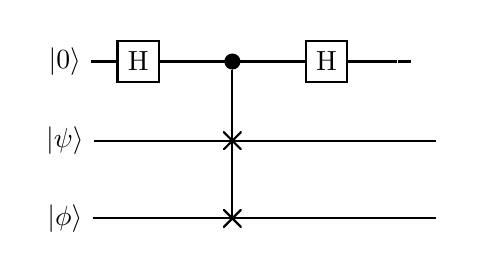
\begin{tikzpicture}[thick,cross/.style={path picture={ 
  \draw[black]
(path picture bounding box.south) -- (path picture bounding box.north);
}},swap/.style={path picture={ 
  \draw[black]
(path picture bounding box.south west) -- (path picture bounding box.north east) (path picture bounding box.south east) -- (path picture bounding box.north west);
}}]

    % `operator' will only be used by most gates.
    % `cnot' will refer to CNOT gates.
    % `phase' is used for controlled gates.
    \tikzstyle{operator} = [draw,fill=white,minimum size=1.5em]
    \tikzstyle{meter} = [draw,color=white,fill=white,minimum size=1.7em]
    \tikzstyle{cnot} = [draw,cross,circle,minimum size=5pt]
    \tikzstyle{phase} = [draw,fill,shape=circle,minimum size=5pt,inner sep=0pt]
    %
    \matrix[row sep=0.4cm, column sep=0.8cm] (circuit) {

    % First row.
    \node (q1) {\ket{0}}; &[-0.5cm] 
    \node[operator] (O11) {H}; &
    \node[phase] (P12) {}; &
    \node[operator] (O13) {H}; &
    \node[meter] (M11) {\pgfbox[center,center]{\pgfuseimage{meter}}};\\
    
    % Second row.
    \node (q2) {\ket{\psi}}; &
    &
    \coordinate (swap22);
    \node[swap] (O22) {}; &
    &
    \coordinate (end2); \\

    % Third row.
    \node (q3) {\ket{\phi}}; &
    &
    \coordinate (swap32);
    \node[swap] (O32) {}; &
    &
    \coordinate (end3); \\
    };

    \begin{pgfonlayer}{background}
        % Draw lines.
        \draw[thick] (q1) -- (M11)  (q2) -- (end2) (q3) -- (end3) (P12) -- (swap22) (swap22) -- (swap32);
    \end{pgfonlayer}
    %
    \end{tikzpicture}
\end{document}
